\documentclass[12pt,a4paper]{article}
\usepackage{hyperref} % Use the Charter font for the document text
%\usepackage[UTF8]{ctex}
\usepackage{fullpage}
\usepackage{amsfonts,amssymb,amsmath}
\usepackage{mathtools}
\usepackage{tikz-cd}
\usepackage{tikz}

\usepackage{alltt}
\usepackage{amsfonts}
\usepackage{amsmath}
\usepackage{amssymb}
\usepackage{amsthm}
\usepackage{booktabs}
\usepackage{caption}
\usepackage{enumitem}
\usepackage{fancyhdr}
\usepackage{graphicx}
\usepackage{mathdots}
\usepackage{mathtools}
\usepackage{microtype}
\usepackage{multirow}
\usepackage{pdflscape}
\usepackage{pgfplots}
\usepackage{siunitx}
\usepackage{slashed}
\usepackage{tabularx}
\usepackage{tikz}
\usepackage{tkz-euclide}
\usepackage[normalem]{ulem}
\usepackage[all]{xy}
\usepackage{imakeidx}

\newcommand{\bA}{\ensuremath{\mathbb{A}}}
\newcommand{\bB}{\ensuremath{\mathbb{B}}}
\newcommand{\bC}{\ensuremath{\mathbb{C}}}
\newcommand{\bD}{\ensuremath{\mathbb{D}}}
\newcommand{\bE}{\ensuremath{\mathbb{E}}}
\newcommand{\bF}{\ensuremath{\mathbb{F}}}
\newcommand{\bG}{\ensuremath{\mathbb{G}}}
\newcommand{\bH}{\ensuremath{\mathbb{H}}}
\newcommand{\bI}{\ensuremath{\mathbb{I}}}
\newcommand{\bJ}{\ensuremath{\mathbb{J}}}
\newcommand{\bK}{\ensuremath{\mathbb{K}}}
\newcommand{\bL}{\ensuremath{\mathbb{L}}}
\newcommand{\bM}{\ensuremath{\mathbb{M}}}
\newcommand{\bN}{\ensuremath{\mathbb{N}}}
\newcommand{\bO}{\ensuremath{\mathbb{O}}}
\newcommand{\bP}{\ensuremath{\mathbb{P}}}
\newcommand{\bQ}{\ensuremath{\mathbb{Q}}}
\newcommand{\bR}{\ensuremath{\mathbb{R}}}
\newcommand{\bS}{\ensuremath{\mathbb{S}}}
\newcommand{\bT}{\ensuremath{\mathbb{T}}}
\newcommand{\bU}{\ensuremath{\mathbb{U}}}
\newcommand{\bV}{\ensuremath{\mathbb{V}}}
\newcommand{\bW}{\ensuremath{\mathbb{W}}}
\newcommand{\bX}{\ensuremath{\mathbb{X}}}
\newcommand{\bY}{\ensuremath{\mathbb{Y}}}
\newcommand{\bZ}{\ensuremath{\mathbb{Z}}}


%
%\parskip=1em
%\parindent=0.3in
%\setlength\oddsidemargin{0.5in} \setlength\evensidemargin{0.5in}
%\setlength\textwidth{5.5in}
%
%\hfuzz6pt % Don't bother to report over-full boxes if over-edge is < 6pt
%
%\newlength{\defbaselineskip}
%\setlength{\defbaselineskip}{\baselineskip}
%\newcommand{\setlinespacing}[1]%
%           {\setlength{\baselineskip}{#1 \defbaselineskip}}
%\newcommand{\doublespacing}{\setlength{\baselineskip}%
%                           {2.0 \defbaselineskip}}
%\newcommand{\singlespacing}{\setlength{\baselineskip}{\defbaselineskip}}
%
%\newcommand{\properpagestyle}{\pagestyle{myheadings}\markboth{}{}\markright{}}




\def\Ric{\mathop{\rm Ric}}
\def\cRic{\mathop{\stackrel{\circ}{\Ric}}}
\def\Scal{\mathop{\rm R}}
\def\scL{\mathop{\mathcal L}}
\def\Hess{\mathop{\rm Hess}}
\def\bt{\mathop{\bar\tau}}
\def\dist{\mathop{\rm dist}}
\def\Cut{\mathop{\rm Cut}}
\def\Riem{\mathop{\rm Rm}}
\def\scal{\mathop{\rm scal}}
\def\Sec{\mathop{\rm Sec}}
\def\Diam{\mathop{\rm Diam}}
\def\CS{\mathop{\rm C_S}}
\def\V{\mathop{\rm V}}
\def\Vol{\mathop{\rm Vol}}
\def\Area{\mathop{\rm Area}}
\def\VR{\mathop{\rm VR}}
\def\supp{\mathop{\rm supp}}
\def\div{\mathop{\rm div}}
\def\inj{\mathop{\rm inj}}
\def\diam{\mathop{\rm diam}}
\def\Id{\mathop{\rm Id}}
\def\RRR{\mathop{\mathcal{R}}}
\def\MMM{\mathop{\mathcal{M}}}
\def\HHH{\mathop{\mathcal{H}}}
\def\VVV{\mathop{\mathcal{V}}}
\def\FF{\mathop{\mathbb{F}}}
\def\RR{\mathop{\mathbb{R}}}
\def\QQ{\mathop{\mathbb{Q}}}
\def\CC{\mathop{\mathbb{C}}}
\def\ZZ{\mathop{\mathbb{Z}}}
\def\SS{\mathop{\mathbb{S}}}
\def\SSS{\mathop{\mathcal{S}}}
\def\PP{\mathop{\mathbb{P}}}
\def\End{\mathop{\rm End}}
\def\Aut{\mathop{\rm Aut}}
\def\Ad{\mathop{\rm Ad}}
\def\ad{\mathop{\rm ad}}
\def\hht{\mathop{\rm ht}}
\def\gl{\mathop{\mathfrak{gl}}}
\def\ssl{\mathop{\mathfrak{sl}}}
\def\TP{\mathop{\mathcal{TP}}}
\def\PPP{\mathop{\mathcal{P}}}
\def\gggg{\mathop{\mathfrak{g}}}
\def\ffff{\mathop{\mathfrak{f}}}
\def\OO{\mathop{\mathcal{O}}}
\def\oo{\mathop{\mathfrak{o}}}
\def\GG{\mathop{\mathcal{G}}}
\def\WWW{\mathop{\mathcal{W}}}
\def\Rad{\mathop{\rm Rad}}
\def\Der{\mathop{\rm Der}}
\def\Ker{\mathop{\rm Ker}}
\def\Im{\mathop{\rm Im}}

\def\be{\begin{eqnarray}}
\def\ee{\end{eqnarray}}
\def\beg{\begin{eqnarray*}}
\def\ees{\end{eqnarray*}}


%\newcommand{\qed}{\hfill$\Box$}
\theoremstyle{definition}
\newtheorem*{aim}{Aim}
\newtheorem*{axiom}{Axiom}
\newtheorem*{claim}{Claim}
\newtheorem*{cor}{Corollary}
\newtheorem*{conjecture}{Conjecture}
\newtheorem*{defi}{Definition}
\newtheorem*{eg}{Example}
\newtheorem*{ex}{Exercise}
\newtheorem*{fact}{Fact}
\newtheorem*{law}{Law}
\newtheorem*{lemma}{Lemma}
\newtheorem*{notation}{Notation}
\newtheorem*{prop}{Proposition}
\newtheorem*{question}{Question}
\newtheorem*{thm}{Theorem}





% Maths symbols
\newcommand{\abs}[1]{\left\lvert #1\right\rvert}
%\newcommand\ad{\mathrm{ad}}
\newcommand\AND{\mathsf{AND}}
\newcommand\Art{\mathrm{Art}}
\newcommand{\Bilin}{\mathrm{Bilin}}
\newcommand{\bket}[1]{\left\lvert #1\right\rangle}
\newcommand{\B}{\mathcal{B}}
\newcommand{\bolds}[1]{{\bfseries #1}}
\newcommand{\brak}[1]{\left\langle #1 \right\rvert}
\newcommand{\braket}[2]{\left\langle #1\middle\vert #2 \right\rangle}
\newcommand{\bra}{\langle}
\newcommand{\cat}[1]{\mathsf{#1}}
\newcommand{\C}{\mathbb{C}}
\newcommand{\CP}{\mathbb{CP}}
\newcommand{\cU}{\mathcal{U}}
%\newcommand{\Der}{\mathrm{Der}}
\newcommand{\D}{\mathrm{D}}
\newcommand{\dR}{\mathrm{dR}}
\newcommand{\E}{\mathbb{E}}
\newcommand{\F}{\mathbb{F}}
\newcommand{\Frob}{\mathrm{Frob}}
%\newcommand{\GG}{\mathbb{G}}
%\newcommand{\gl}{\mathfrak{gl}}
\newcommand{\GL}{\mathrm{GL}}
\newcommand{\G}{\mathcal{G}}
\newcommand{\Gr}{\mathrm{Gr}}
\newcommand{\haut}{\mathrm{ht}}
\newcommand{\Hol}{\mathrm{Hol}}
\newcommand{\hol}{\mathfrak{hol}}
%\newcommand{\Id}{\mathrm{Id}}
\newcommand{\ket}{\rangle}
\newcommand{\lie}[1]{\mathfrak{#1}}
\newcommand{\Mat}{\mathrm{Mat}}
\newcommand{\N}{\mathbb{N}}
\newcommand{\norm}[1]{\left\lVert #1\right\rVert}
\newcommand{\normalorder}[1]{\mathop{:}\nolimits\!#1\!\mathop{:}\nolimits}
\newcommand{\NOT}{\mathsf{NOT}}
\newcommand{\op}{\mathrm{op}}
\newcommand{\Oc}{\mathcal{O}}
\newcommand{\Or}{\mathrm{O}}
\newcommand\OR{\mathsf{OR}}
\newcommand{\ort}{\mathfrak{o}}
\newcommand{\PGL}{\mathrm{PGL}}
\newcommand{\ph}{\,\cdot\,}
\newcommand{\pr}{\mathrm{pr}}
\newcommand{\Prob}{\mathbb{P}}
\newcommand{\PSL}{\mathrm{PSL}}
\newcommand{\Ps}{\mathcal{P}}
\newcommand{\PSU}{\mathrm{PSU}}
\newcommand{\pt}{\mathrm{pt}}
\newcommand{\qeq}{\mathrel{``{=}"}}
\newcommand{\Q}{\mathbb{Q}}
\newcommand{\R}{\mathbb{R}}
\newcommand{\RP}{\mathbb{RP}}
\newcommand{\Rs}{\mathcal{R}}
\newcommand{\SL}{\mathrm{SL}}
\newcommand{\so}{\mathfrak{so}}
\newcommand{\SO}{\mathrm{SO}}
\newcommand{\Spin}{\mathrm{Spin}}
\newcommand{\Sp}{\mathrm{Sp}}
\newcommand{\su}{\mathfrak{su}}
\newcommand{\SU}{\mathrm{SU}}
\newcommand{\term}[1]{\textbf{#1}\index{#1}}
\newcommand{\T}{\mathbb{T}}
\newcommand{\tv}[1]{|#1|}
\newcommand{\U}{\mathrm{U}}
\newcommand{\uu}{\mathfrak{u}}
\newcommand{\Vect}{\mathrm{Vect}}
\newcommand{\wsto}{\stackrel{\mathrm{w}^*}{\to}}
\newcommand{\wt}{\mathrm{wt}}
\newcommand{\wto}{\stackrel{\mathrm{w}}{\to}}
\newcommand{\Z}{\mathbb{Z}}
\renewcommand{\d}{\mathrm{d}}
\renewcommand{\H}{\mathbb{H}}
\renewcommand{\P}{\mathbb{P}}
\renewcommand{\sl}{\mathfrak{sl}}
\renewcommand{\vec}[1]{\boldsymbol{\mathbf{#1}}}
%\renewcommand{\F}{\mathcal{F}}

\let\Im\relax
\let\Re\relax

\DeclareMathOperator{\adj}{adj}
\DeclareMathOperator{\Ann}{Ann}
\DeclareMathOperator{\area}{area}
%\DeclareMathOperator{\Aut}{Aut}
\DeclareMathOperator{\Bernoulli}{Bernoulli}
\DeclareMathOperator{\betaD}{beta}
\DeclareMathOperator{\bias}{bias}
\DeclareMathOperator{\binomial}{binomial}
\DeclareMathOperator{\card}{card}
\DeclareMathOperator{\ccl}{ccl}
\DeclareMathOperator{\Char}{char}
\DeclareMathOperator{\ch}{ch}
\DeclareMathOperator{\cl}{cl}
\DeclareMathOperator{\cls}{\overline{\mathrm{span}}}
\DeclareMathOperator{\coker}{coker}
\DeclareMathOperator{\conv}{conv}
\DeclareMathOperator{\corr}{corr}
\DeclareMathOperator{\cosec}{cosec}
\DeclareMathOperator{\cosech}{cosech}
\DeclareMathOperator{\cov}{cov}
\DeclareMathOperator{\covol}{covol}
\DeclareMathOperator{\diag}{diag}
%\DeclareMathOperator{\diam}{diam}
\DeclareMathOperator{\Diff}{Diff}
\DeclareMathOperator{\disc}{disc}
\DeclareMathOperator{\dom}{dom}
%\DeclareMathOperator{\End}{End}
\DeclareMathOperator{\energy}{energy}
\DeclareMathOperator{\erfc}{erfc}
\DeclareMathOperator{\erf}{erf}
\DeclareMathOperator*{\esssup}{ess\,sup}
\DeclareMathOperator{\ev}{ev}
\DeclareMathOperator{\Ext}{Ext}
\DeclareMathOperator{\fst}{fst}
\DeclareMathOperator{\Fit}{Fit}
\DeclareMathOperator{\fix}{fix}
\DeclareMathOperator{\Frac}{Frac}
\DeclareMathOperator{\Gal}{Gal}
\DeclareMathOperator{\gammaD}{gamma}
\DeclareMathOperator{\gr}{gr}
\DeclareMathOperator{\hcf}{hcf}
\DeclareMathOperator{\Hom}{Hom}
\DeclareMathOperator{\id}{id}
\DeclareMathOperator{\Image}{image}
\DeclareMathOperator{\Im}{Im}
\DeclareMathOperator{\Ind}{Ind}
\DeclareMathOperator{\Int}{Int}
\DeclareMathOperator{\Isom}{Isom}
\DeclareMathOperator{\lcm}{lcm}
\DeclareMathOperator{\length}{length}
\DeclareMathOperator{\Lie}{Lie}
\DeclareMathOperator{\like}{like}
\DeclareMathOperator{\Lk}{Lk}
\DeclareMathOperator{\Maps}{Maps}
\DeclareMathOperator{\mse}{mse}
\DeclareMathOperator{\multinomial}{multinomial}
\DeclareMathOperator{\orb}{orb}
\DeclareMathOperator{\ord}{ord}
\DeclareMathOperator{\otp}{otp}
\DeclareMathOperator{\Poisson}{Poisson}
\DeclareMathOperator{\poly}{poly}
\DeclareMathOperator{\rank}{rank}
\DeclareMathOperator{\rel}{rel}
%\DeclareMathOperator{\Rad}{Rad}
\DeclareMathOperator{\Re}{Re}
\DeclareMathOperator*{\res}{res}
\DeclareMathOperator{\Res}{Res}
%\DeclareMathOperator{\Ric}{Ric}
\DeclareMathOperator{\rk}{rk}
\DeclareMathOperator{\Rees}{Rees}
\DeclareMathOperator{\Root}{Root}
\DeclareMathOperator{\sech}{sech}
\DeclareMathOperator{\sgn}{sgn}
\DeclareMathOperator{\snd}{snd}
\DeclareMathOperator{\Spec}{Spec}
\DeclareMathOperator{\spn}{span}
\DeclareMathOperator{\stab}{stab}
\DeclareMathOperator{\St}{St}
%\DeclareMathOperator{\supp}{supp}
\DeclareMathOperator{\Syl}{Syl}
\DeclareMathOperator{\Sym}{Sym}
\DeclareMathOperator{\tr}{tr}
\DeclareMathOperator{\Tr}{Tr}
\DeclareMathOperator{\var}{var}
\DeclareMathOperator{\vol}{vol}
\usetikzlibrary{knots}




\pgfarrowsdeclarecombine{twolatex'}{twolatex'}{latex'}{latex'}{latex'}{latex'}
\tikzset{->/.style = {decoration={markings,
                                  mark=at position 1 with {\arrow[scale=2]{latex'}}},
                      postaction={decorate}}}
\tikzset{<-/.style = {decoration={markings,
                                  mark=at position 0 with {\arrowreversed[scale=2]{latex'}}},
                      postaction={decorate}}}
\tikzset{<->/.style = {decoration={markings,
                                   mark=at position 0 with {\arrowreversed[scale=2]{latex'}},
                                   mark=at position 1 with {\arrow[scale=2]{latex'}}},
                       postaction={decorate}}}
\tikzset{->-/.style = {decoration={markings,
                                   mark=at position #1 with {\arrow[scale=2]{latex'}}},
                       postaction={decorate}}}
\tikzset{-<-/.style = {decoration={markings,
                                   mark=at position #1 with {\arrowreversed[scale=2]{latex'}}},
                       postaction={decorate}}}
\tikzset{->>/.style = {decoration={markings,
                                  mark=at position 1 with {\arrow[scale=2]{latex'}}},
                      postaction={decorate}}}
\tikzset{<<-/.style = {decoration={markings,
                                  mark=at position 0 with {\arrowreversed[scale=2]{twolatex'}}},
                      postaction={decorate}}}
\tikzset{<<->>/.style = {decoration={markings,
                                   mark=at position 0 with {\arrowreversed[scale=2]{twolatex'}},
                                   mark=at position 1 with {\arrow[scale=2]{twolatex'}}},
                       postaction={decorate}}}
\tikzset{->>-/.style = {decoration={markings,
                                   mark=at position #1 with {\arrow[scale=2]{twolatex'}}},
                       postaction={decorate}}}
\tikzset{-<<-/.style = {decoration={markings,
                                   mark=at position #1 with {\arrowreversed[scale=2]{twolatex'}}},
                       postaction={decorate}}}


\tikzset{circ/.style = {fill, circle, inner sep = 0, minimum size = 3}}
\tikzset{scirc/.style = {fill, circle, inner sep = 0, minimum size = 1.5}}
\tikzset{mstate/.style={circle, draw, blue, text=black, minimum width=0.7cm}}

\tikzset{eqpic/.style={baseline={([yshift=-.5ex]current bounding box.center)}}}
\tikzset{commutative diagrams/.cd,cdmap/.style={/tikz/column 1/.append style={anchor=base east},/tikz/column 2/.append style={anchor=base west},row sep=tiny}}


\definecolor{mblue}{rgb}{0.2, 0.3, 0.8}
\definecolor{morange}{rgb}{1, 0.5, 0}
\definecolor{mgreen}{rgb}{0.1, 0.4, 0.2}
\definecolor{mred}{rgb}{0.5, 0, 0}


%\title{ Lecture 4}
\begin{document}\thispagestyle{empty}

\centerline{\Large \bf Lecture 7}

\centerline{\Large \bf Nakahara section 3}



\section{Simplicial complexes}

The relevance is that these can be used to define simplexes (which are simple, as opposed to complexes).
\begin{defi}[$n$-simplex]
  An \textbf{$n$-simplex} is the convex hull of $(n + 1)$ affinely independent points $a_0, \cdots, a_n \in \bR^m$, i.e.\ the set
  \[
    \sigma = \bra a_0, \cdots, a_n\ket = \left\{\sum_{i = 0} t_i a_i : \sum_{i = 0}^n t_i = 1,t_i \geq 0\right\}.
  \]
  The points $a_0, \cdots, a_n$ are the \textbf{vertices}, and are said to \textbf{span} $\sigma$. The $(n + 1)$ tuples $(t_0, \cdots, t_n)$ are called the \textbf{barycentric coordinates} for the point $\sum t_i a_i$.
  
  

  We often denote an oriented simplex as $\sigma$, and then $\bar{\sigma}$ denotes the same simplex with the opposite orientation.
\end{defi}

Some examples are as follows. When $n=0$, it is a point. $n=1$, it is a line.

  \begin{minipage}[b]{2.5cm}  
 \begin{center}
    \begin{tikzpicture}
      \node [circ] at (0,1) {};
        \node at (0,0) {$n=0$};
    \end{tikzpicture}  
  \end{center}
      \end{minipage}
  \begin{minipage}[b]{3.5cm} 
   \begin{center}
    \begin{tikzpicture}
      \node [circ] at (0, 0) {};
      \node [circ] at (2, 0) {};
      \draw (0, 0) -- (2, 0);
              \node at (1,-1) {$n=1$};
    \end{tikzpicture}
  \end{center}
      \end{minipage}
  \begin{minipage}[b]{3.5cm}
  \begin{center}
    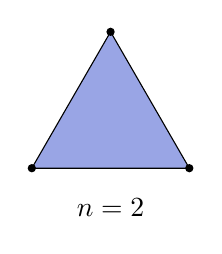
\begin{tikzpicture}
      \draw [fill=mblue, fill opacity=0.5] (0, 0) -- (2, 0) -- (1, 1.732) -- cycle;
      \node [circ] at (0, 0) {};
      \node [circ] at (2, 0) {};
      \node [circ] at (1, 1.732) {};
                    \node at (1,-.5) {$n=2$};
    \end{tikzpicture}
  \end{center}
    \end{minipage}
  \begin{minipage}[b]{3.5cm}
  \begin{center}
    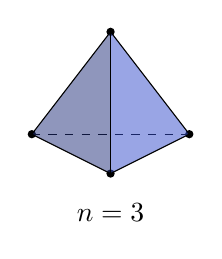
\begin{tikzpicture}
      \node [circ] at (0, 0) {};
      \node [circ] at (2, 0) {};
      \node [circ] at (1, -0.5) {};
      \node [circ] at (1, 1.3) {};
      \draw [dashed] (0, 0) -- (2, 0);
      \fill [mblue, opacity=0.5] (2, 0) -- (1, -0.5) -- (1, 1.3) -- cycle;
      \fill [mblue!60!black, opacity=0.5] (0, 0) -- (1, -0.5) -- (1, 1.3) -- cycle;
      \draw (2, 0) -- (1, -0.5) -- (0, 0);
      \draw (0, 0) -- (1, 1.3) -- (2, 0);
      \draw (1, 1.3) -- (1, -0.5);
                          \node at (1,-1) {$n=3$};
    \end{tikzpicture}
  \end{center}
  \end{minipage}

  A \textbf{face} of a simplex is a subset (or subsimplex) spanned by a subset of the vertices. The \textbf{boundary} is the union of the proper faces, and the \textbf{interior} is the complement of the boundary. The boundary of $\sigma$ is usually denoted by $\partial \sigma$, while the interior is denoted by $\mathring{\sigma}$, and we write $\tau \leq \sigma$ when $\tau$ is a face of $\sigma$. In particular, the interior of a vertex is the vertex itself. Note that this notion of interior and boundary is distinct from the topological notion of boundary.
  
  
  
  

\begin{eg}
  The \textbf{standard $n$-simplex} is spanned by the basis vectors $\{\mathbf{e}_1, \cdots, \mathbf{e}_n\}$ in $\bR^{n + 1}$. For example, when $n = 2$, we get the following:
  \begin{center}
    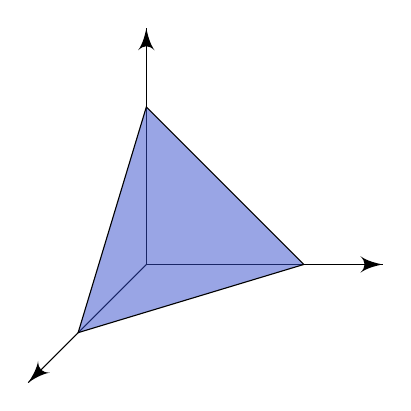
\begin{tikzpicture}
      \draw [->] (0, 0) -- (3, 0);
      \draw [->] (0, 0) -- (0, 3);
      \draw [->] (0, 0) -- (-1.5, -1.5);

      \draw [fill=mblue, fill opacity=0.5] (0, 2) -- (2, 0) -- (-.866, -0.866) -- cycle;
    \end{tikzpicture}
  \end{center}
\end{eg}

We will now glue simplices together to build \textbf{complexes}, or \textbf{simplicial complexes}.

\begin{defi}
  A \textbf{simplicial complex} is a finite set $K$ of simplices in $\bR^n$ such that
  \begin{enumerate}
    \item If $\sigma \in K$ and $\tau$ is a face of $\sigma$, then $\tau \in K$.
    \item If $\sigma, \tau \in K$, then $\sigma \cap \tau$ is either empty or a face of both $\sigma$ and $\tau$.
  \end{enumerate}
\end{defi}



\begin{eg}
  This is a simplicial complex:
  \begin{center}
    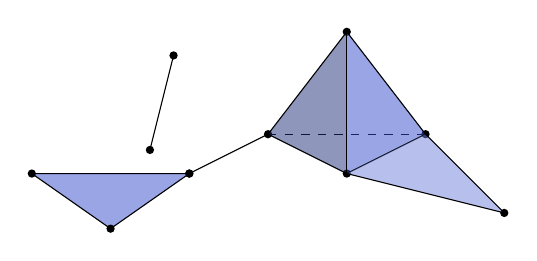
\begin{tikzpicture}
      \node [circ] at (0, 0) {};
      \node [circ] at (2, 0) {};
      \node [circ] at (3, -1) {};
      \node [circ] at (1, -0.5) {};
      \node [circ] at (1, 1.3) {};
      \node [circ] at (-1, -0.5) {};
      \draw [dashed] (0, 0) -- (2, 0);
      \fill [mblue, opacity=0.5] (2, 0) -- (1, -0.5) -- (1, 1.3) -- cycle;
      \fill [mblue!60!black, opacity=0.5] (0, 0) -- (1, -0.5) -- (1, 1.3) -- cycle;
      \draw (2, 0) -- (1, -0.5) -- (0, 0);
      \draw (0, 0) -- (1, 1.3) -- (2, 0);
      \draw (1, 1.3) -- (1, -0.5);
      \draw [fill=mblue!70!white, fill opacity=0.5] (2, 0) -- (3, -1) -- (1, -0.5);

      \draw (0, 0) -- (-1, -0.5);
      \draw [fill=mblue, fill opacity=0.5] (-3, -0.5) -- (-1, -0.5) -- (-2, -1.2) -- cycle;
      \node [circ] at (-3, -0.5) {};
      \node [circ] at (-1, -0.5) {};
      \node [circ] at (-2, -1.2) {};

      \draw (-1.5, -0.2) node [circ] {} -- (-1.2, 1) node [circ] {};
    \end{tikzpicture}
  \end{center}
\end{eg}
Technically, a simplicial complex is defined to be a set of simplices, which is just collections of points. It is not a subspace of $\bR^n$.  The \textbf{polyhedron} defined by $K$ is the union of the simplices in $K$, and denoted by $|K|$.  The \textbf{dimension} of $K$ is the highest dimension of a simplex of $K$. The \textbf{$d$-skeleton} $K^{(d)}$ of $K$ is the union of the $n$-simplices in $K$ for $n \leq d$.
  A \textbf{triangulation} of a space $X$ is a homeomorphism $h: |K| \to X$, where $K$ is some simplicial complex.


\begin{eg}
  Let $\sigma$ be the standard $n$-simplex. The boundary $\partial \sigma$ is homeomorphic to $S^{n - 1}$ (e.g.\ the boundary of a (solid) triangle is the boundary of the triangle, which is also a circle) . This is called the \textbf{simplicial $(n - 1)$ sphere}.
\end{eg}

We can also triangulate our $S^n$ in a different way:
\begin{eg}
  In $\bR^{n + 1}$, consider the simplices $ \bra \pm \mathbf{e}_0, \cdots, \pm \mathbf{e}_n\ket$ for each possible combination of signs. So we have $2^{n + 1}$ simplices in total. Then their union defines a simplicial complex $K$, and
  \[
    |K| \cong S^n.
  \]
  \begin{center}
    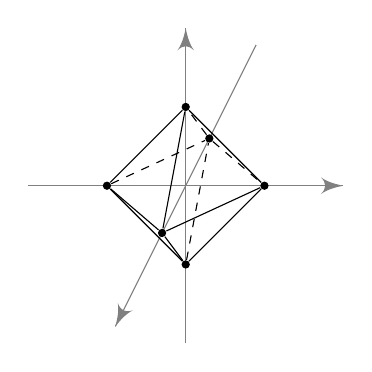
\begin{tikzpicture}
      \draw [gray, ->] (-2, 0) -- (2, 0);
      \draw [gray, ->] (0, -2) -- (0, 2);
      \draw [gray, ->] (0.894, 1.788) -- (-0.894, -1.788);

      \node [circ] (x1) at (1, 0) {};
      \node [circ] (x2) at (-1, 0) {};
      \node [circ] (z1) at (0, 1) {};
      \node [circ] (z2) at (0, -1) {};
      \node [circ] (y1) at (-0.3, -0.6) {};
      \node [circ] (y2) at (0.3, 0.6) {};

      \draw (x1) -- (y1) -- (z1) -- (x1) -- (z2) -- (y1) -- (x2) -- (z1);
      \draw (z2) -- (x2);
      \draw [dashed] (x2) -- (y2) -- (x1);
      \draw [dashed] (z2) -- (y2) -- (z1);
    \end{tikzpicture}
  \end{center}
\end{eg}
The nice thing about this triangulation is that the simplicial complex is invariant under the antipodal map. So not only can we think of this as a triangulation of the sphere, but a triangulation of $\RP^n$ as well.





    An \textbf{oriented $n$-simplex} in a simplicial complex $K$ is an $n + 1$-tuple $(a_0, \cdots, a_n)$ of vertices $a_i \in V_k$ such that $\bra a_0, \cdots, a_n\ket \in K$, where we think of two $n + 1$ tuples $(a_0, \cdots, a_n)$ and $(a_{\pi(0)}, \cdots, a_{\pi(n)})$ as the same \textbf{oriented} simplex if $\pi \in S^n$ is an \textbf{even} permutation.
    
    
    
\begin{defi}[Chain group $C_n(K)$]
  Let $K$ be a simplicial complex. 
  Let $\{\sigma_1, \cdots, \sigma_\ell\}$ be the set of $n$-simplices of $K$ with orientation. Then we define $C_n(K)$ be the free abelian group with basis $\{\sigma_1, \cdots, \sigma_\ell\}$, i.e.\ $C_n(K) \cong \Z^\ell$.
\end{defi}


  We define \textbf{boundary homomorphisms}
  \[
    \partial_n: C_n(K) \to C_{n - 1}(K)
  \]
  by
  \[
    (a_0, \cdots, a_n) \mapsto \sum_{i = 0}^n (-1)^i (a_0, \cdots, \hat{a}_i, \cdots, a_n),
  \]
  where $(a_0, \cdots, \hat{a}_i, \cdots, a_n) = (a_0, \cdots, a_{i - 1}, a_{i + 1}, a_n)$ is the simplex with $a_i$ removed. We can show that $\partial_{n+1}\cdot \partial_n=0$.




We will develop some formalism to help us compute homology groups $H_k(K)$ in lots of examples. 
\begin{defi}[Chain complex and differentials]
  A \textbf{chain complex} $C_{\bullet}$ is a sequence of chain groups $C_0, C_1, C_2, \cdots$ equipped with boundary maps $\partial_n: C_n \to C_{n - 1}$ such that $\partial_{n - 1} \circ \partial_n = 0$ for all $n$.
\end{defi}
\[
  \begin{tikzcd}
  \cdots \ar [r, "\partial_3"'] & C_2 \ar [r, "\partial_2"']   &   C_1 \ar [r, "\partial_1"'] &C_0 \ar[r, "\partial_0"'] &    0 
  \end{tikzcd}
\]

As in the de Rham cohomology, we define the \textbf{$n$-cycles} is 
  \[
    Z_n(C) = \Ker \partial_n.
  \]
  The \textbf{$n$-boundaries} is
  \[
    B_n(C) = \Im \partial_{n+1}.
  \]
Then,  the \textbf{$n$-th homology group} of $C_{\bullet}$ is defined to be
  \[
    H_n(C) = \frac{\Ker \partial_n}{\Im \partial_{n + 1}} = \frac{Z_n(C)}{B_n(C)}.
  \]
  
  
Let  $K\to X$ be a triangulation of an $n$-dimensional compact oriented closed connected manifold $X$. Then, the $n$-th homology is $H_n(K,\Z)\cong \Z$ and its generator is denoted by $[X]$ and called the \textbf{fundamental  class}. 
  

  The \textbf{Euler characteristic} of a triangulated space $h: |K| \to X$ is the alternative sum of real-valued homology groups of $|K|$
  \[
    \chi(X) = \sum_{i \geq 0} (-1)^i \dim_\R H_i(K; \R).
  \]
As we will see below, this  depends only on the homotopy type of $X$. 

\begin{eg}
  Let $K$ be the standard simplicial $1$-sphere, ie, we have the following in $\R^3$.
  \begin{center}
    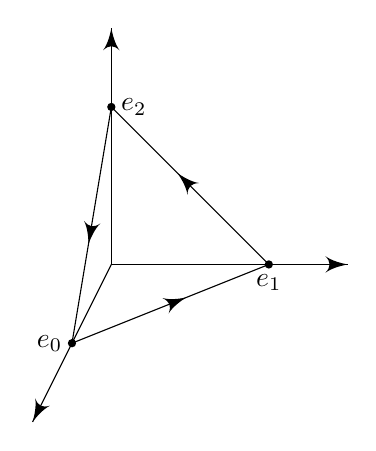
\begin{tikzpicture}
      \draw [->] (0, 0) -- (3, 0);
      \draw [->] (0, 0) -- (0, 3);
      \draw [->] (0, 0) -- (-1, -2);

      \draw [->-=0.58] (2, 0) -- (0, 2);
      \draw [->-=0.58] (0, 2) -- (-0.5, -1);
      \draw [->-=0.58] (-0.5, -1) -- (2, 0);

      \node [left] at (-0.5, -1) {$e_0$};
      \node [below] at (2, 0) {$e_1$};
      \node [right] at (0, 2) {$e_2$};

      \node [circ] at (-0.5, -1) {};
      \node [circ] at (2, 0) {};
      \node [circ] at (0, 2) {};
    \end{tikzpicture}
  \end{center}
  Our simplices are thus
  \[
    K = \{\bra e_0\ket, \bra e_1\ket, \bra e_2\ket, \bra e_0, e_1\ket, \bra e_1, e_2\ket, \bra e_2, e_0\ket\}.
  \]
  Our chain groups are
  \begin{align*}
    C_0(K) &= \bra (e_0), (e_1), (e_2)\ket \cong \Z^3\\
    C_1(K) &= \bra (e_0, e_1), (e_1, e_2), (e_2, e_0)\ket \cong \Z^3.
  \end{align*}
  All other chain groups are zero. Note that our notation is slightly confusing here, since the brackets $\bra \ph \ket$ can mean the simplex spanned by the vertices, or the group generated by certain elements. However, you are probably clueful enough to distinguish the two use cases.

  Hence, the only non-zero boundary map is
  \[
    \partial_1: C_1(K) \to C_0(K).
  \]
  We can write down its matrix with respect to the given basis.
  \[
    \begin{pmatrix}
      -1 & 0 & 1\\
      1 & -1 & 0\\
      0 & 1 & -1
    \end{pmatrix}
  \]
  We have now everything we need to know about the homology groups, and we just need to do some linear algebra to figure out the image and kernel, and thus the homology groups. We have
  \[
    H_0(K) = \frac{\Ker (\partial_0: C_0(K) \to C_{-1}(K))}{\Im (\partial_1: C_1(K) \to C_0(K))} \cong \frac{C_0(K)}{\Im \partial_1} \cong \frac{\Z^3}{\Im \partial_1}.
  \]
  After doing some row operations with our matrix, we see that the image of $\partial_1$ is a two-dimensional subspace generated by the image of two of the edges. Hence we have
  \[
    H_0(K) = \Z.
  \]
  What does this $H_0(\Z)$ represent? We initially said that $H_k(K)$ should represent the $k$-dimensional holes, but when $k = 0$, this is simpler. As for $\pi_0$, $H_0$ just represents the path components of $K$. We interpret this to mean $K$ has one path component. In general, if $K$ has $r$ path components, then we expect $H_0(K)$ to be $\Z^r$.

  Similarly, we have
  \[
    H_1(K) = \frac{\Ker \partial_1}{\Im \partial_2} \cong \Ker \partial_1.
  \]
  It is easy to see that in fact we have
  \[
    \Ker \partial_1 = \bra (e_0, e_1) + (e_1, e_2) + (e_2, e_0)\ket \cong \Z.
  \]
  So we also have
  \[
    H_1(K) \cong \Z.
  \]
  We see that this $H_1(K)$ is generated by precisely the single loop in the triangle. The fact that $H_1(K)$ is non-trivial means that we do indeed have a hole in the middle of the circle.
\end{eg}

We can also consider a map between two simplicial complexes.

\begin{defi}[Simplicial map]
  A \textbf{simplicial map} $f: K \to L$ is a function $f: V_K \to V_L$ such that if $\bra a_0, \cdots, a_n\ket$ is a simplex in $K$, then $\{f(a_0), \cdots, f(a_n)\}$ spans a simplex of $L$.
\end{defi}


Given triangulations $|K|\to X$ and $|L|\to Y$ for manifolds $X$ and $Y$ and a continuous map $f:X\to Y$, we can ``approximate'' $f$ by a simplicial map $g:K\to L$. (See Hatcher's book from p.177 for more detail.)

In fact, a simplicial map $f$ induces a map between simplicial complexes.



\begin{defi}[Chain map]
  A chain map $f_{\bullet}: C_{\bullet}\to D_{\bullet}$ is a sequence of homomorphisms $f_n: C_n \to D_n$ such that
  \[
    f_{n - 1} \circ \partial_n = \partial_n \circ f_n
  \]
  for all $n$. In other words, the following diagram commutes:
  \[
    \begin{tikzcd}[row sep=large]
 \cdots \ar [r, "\partial_3"']&  C_2 \ar [r, "\partial_2"'] \ar [d, "f_2"'] &   C_1 \ar [r, "\partial_1"'] \ar[d, "f_1"'] & C_0 \ar[r, "\partial_0"'] \ar[d, "f_0"'] &   0   \\
\cdots \ar [r, "\partial_3"]&  D_2 \ar [r, "\partial_2"] &   D_1 \ar [r, "\partial_1"] & D_0 \ar[r, "\partial_0"] &   0
    \end{tikzcd}
  \]
\end{defi}



%Here, $K$ is always a simplicial complex, and $C_{\bullet} = C_{\bullet}(K)$.

  Let $f: K \to L$ be a simplicial map. Then $f$ induces a chain map $f_{\bullet}: C_{\bullet}(K) \to C_{\bullet}(L)$. Hence it also induces $f_*: H_n (K) \to H_n(L);[c] \mapsto [f(c)]$. In fact, given triangulations $|K|\to X$ and $|L|\to Y$ for homotopically equivalent manifolds $f:X \to Y$ with $f\sim \id$, its simplicial approximation $g:K\to L$ induces an isomorphism $g_*: H_n (K) \cong H_n(L)$.





\section{Mayer-Vietoris sequence}


Here I just give you introduction to a powerful theorem called Mayer-Vietoris sequence to compute homology. For more detail, I refer to Hatcher's book (p.149).

Suppose we have a space $K = M\cup N$, where $M \cap N$ are path-connected.
\begin{center}
  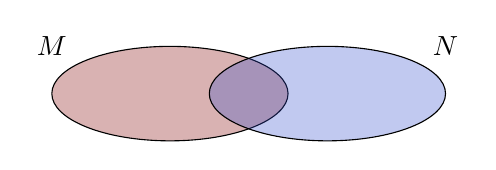
\begin{tikzpicture}
    \draw [fill=mred, fill opacity=0.3] (-1, 0) ellipse (1.5 and 0.6);
    \draw [fill=mblue, fill opacity=0.3] (1, 0) ellipse (1.5 and 0.6);
    \node at (-2.5, 0.6) {$M$};
    \node at (2.5, 0.6) {$N$};
  \end{tikzpicture}
\end{center}
The theorem tells us how to compute the homology of the union $M\cup N$ in terms of those of $M, N$ and $M\cap N$.


\begin{thm}[Mayer-Vietoris theorem]
  Let $K, L, M, N$ be simplicial complexes with $K = M\cup N$ and $L = M\cap N$. We have the following inclusions and maps:
  \[
    \begin{tikzcd}
      L \ar[r, hook, "i"] \ar[d, hook, "j"] & M\ar[d, hook, "k"]\\
      N \ar[r, hook, "\ell"] & K.
    \end{tikzcd}
  \]
  Then there exists some natural homomorphism $p_*: H_n(K) \to H_{n - 1}(L)$ that gives the following long exact sequence:
  \[
    \begin{tikzcd}
      \cdots \ar[r, "p_*"] & H_n(L) \ar[r, "i_* + j_*"] & H_n(M) \oplus H_n(N) \ar[r, "k_* - \ell_*"] & H_n(K)\ar[out=0, in=180, looseness=2, overlay, lld, "p_*"']\\
      & H_{n - 1}(L) \ar[r, "i_* + j_*"] & H_{n - 1}(M) \oplus H_{n - 1}(N) \ar[r, "k_* - \ell_*"] & H_{n - 1}(K) \ar [r] & \cdots\\
      &\cdots \ar[r] & H_0(M) \oplus H_0(N) \ar[r, "k_* - \ell_*"] & H_0(K) \ar [r] & 0
    \end{tikzcd}
  \]
\end{thm}
Here $A \oplus B$ is the direct sum of the two (abelian) groups, which may also be known as the Cartesian product.



\section{de Rham theorem and Poincare duality}
Given a simplicail complex $K$ and its chain group $C_k(K)$, we can define \textbf{cochain group}
$$
C^k(K)=\{ f:C_k(K)\to \Z \  \textrm{homomorphism}\}
$$ 
In addition, we can define \textbf{coboundary} $\delta:C^k(K)\to C^{k+1}(K)$ as $\delta f(c)=f(\partial c)$ were $c\in C_{k+1}(K)$. It is easy to see $\delta\cdot \delta =0$. We can define \textbf{cocycle} $Z^k(K)=\Ker\delta$ and \textbf{coboundary} $B^k(K)=\Im\delta$. The cohomology group of $K$ is defined by 
$$
H^k(K)=Z^k(K)/B^k(K)~.
$$
There exists bilinear map
$$
H_k(K)\otimes H^k(K)\to \Z; ([c],[f])\mapsto f(c)
$$
which is well defined.






\begin{thm}[de Rham]
Let $X$ be a smooth manifold and $|K|\to X$ be its triangulation. Then, we have an isomorphism
$$
H^*_{dR}(X)\cong H^*(K,\bR)~.
$$
\end{thm}



In fact, there is a relation between homology group and cohomology group. A $k$-dimensional oriented submanifold $Y\subset X$ without boundary indeed represents a generator $[Y]\in H_k(X)$. The definition of a submanifold is given in section 5.2.7 of Nakahara. There exists $\eta\in H^{n-k}(X)$ such that
$$
\int_Y \omega =\int_X\omega\wedge \eta
$$
for any $\omega\in H^k(X)$.

\begin{thm}[Poincare duality]
Let $X$ be an $n$-dimensional compact oriented closed manifold. Then, we have an isomorphism
$$
\vartheta: H_{k}(X)\cong H^{n-k}(K,\bR); Y\mapsto \eta
$$
\end{thm}

Using this isomorphism, one can define an \textbf{intersection number} $Y_1\cdot Y_2$ for $Y_1\in H^k(X)$ and $Y_2\in H^{n-k}(X)$.
$$
Y_1\cdot Y_2:=\int_X \eta_1\wedge \eta_2
$$
where $\vartheta(Y_i) =\eta_i$.


\section{Lefschetz fixed point theorem and Poincare-Hopf theorem}
Let $X$ and $Y$ be $n$-dimensional smooth closed oriented manifolds. 
A smooth map $f:X\to Y$ induces an homomorphism $f_*:H_*(X)\to H_*(Y)$. In particular, we define \textbf{mapping degree} of $f$ by 
$$
 f_*([X]):=(\deg f) [Y]~.
$$
In the language of cohomology group, we can define
$$
\deg f:= \frac{\int_{X}f^* \omega} {\int_Y\omega}
$$
where $\omega$ is the volume form of $Y$.

Given two knots $K_1,K_2:S^1\to \bR^3$, we can define $F:K_1\times K_2\to S^2$ by
$$
F(p,q)=\frac{x_1-x_2}{|x_1-x_2|}
$$
Then, we define the \textbf{linking number} of $K_1$ and $K_2$ as
$$
Lk(K_1,K_2):=\deg F=\frac{1}{4\pi}\int_{K_1\times K_2} F^* \omega=\frac{1}{4\pi}\int_{K_1}dx_1^i \int_{K_2} dx_2^j \frac{(x_1-x_2)^k}{|x_1-x_2|^3}\epsilon_{ijk}
$$
where $\omega$ is the volume form of $S^2$.
\begin{figure}[h]\centering
\includegraphics{linking}
\end{figure}

This number was first introduced by Gauss in the study of electromagnetism.  Biot-Savart law tells us that the magnetic field generated by electric current running on $K_1$ with unit strength is
$$
\vec{B}(\vec x)= \frac1{4\pi}\int_{K_1}  \frac{(\vec{x}-\vec {x_1}(t_1))^k\times \frac{d\vec {x_1}}{dt_1} }{|\vec x- \vec x_1|^3}dt_1
$$
Therefore, $Lk(K_1,K_2)$ is the energy which costs to move a magnetic monopole along $K_2$ under this magnetic field. Gauss has noticed that the integral always provides an integer however $K_1$ and $K_2$ are drawn. Moreover, this number stays invariant even though you deform $K_1$ and $K_2$!


Let $X$ be an $n$-dimensional smooth closed oriented manifold. 
We assume that a map $f: X \to X$ has isolated fixed points $f(p)=p$. We define a map $h:S^{n-1}_\epsilon\to S^{n-1}$ by
$$
h(q)=\frac{q-f(q)}{|q-f(q)|}
$$
The index of $f$ at the fixed point $p$ is defined by
$$
\textrm{ind}_p f:=\deg h
$$
We define the \textbf{Lefschetz number} of $f$ as
  \[
    L(f) = \sum_{i \geq 0} (-1)^i \tr(f_*: H_i(X; \R) \to H_i(X; \R)).
  \]

\begin{thm}[Lefschetz fixed point theorem]
Lefschetz number is the sum of indices over isolated fixed points
$$
 L(f)=\sum_{p} \textrm{ind}_p f
$$
\end{thm}
\begin{minipage}[b]{6.5cm}
\includegraphics[width=5.5cm]{vector-fields}
\end{minipage}
\begin{minipage}[b]{8cm}
\includegraphics[width=8.5cm]{vector-field-indices}
\end{minipage}

Let $v$ is a vector field on $X$ and $\varphi_t$ is a flow generated by $v$. Then, the index of a zero point $p$ of $v$ is defined by
$$
\textrm{ind}_p v =\textrm{ind}_p \varphi_t~.
$$
Since the flow $\varphi_t$ is homotopic to the identity $\varphi_t\sim id$, $L(\varphi_t)$ is equal to the Euler characteristic.
$$
    L(\varphi_t) =\sum_{i \geq 0} (-1)^i \tr(id: H_i(X; \R) \to H_i(X; \R)).=\sum_{i \geq 0} (-1)^i \dim H_i(X; \R) =\chi(X)
$$
Therefore, we obtain:
\begin{thm}[Poincare-Hopf theorem]
The Euler characteristics is the sum of indices over isolated fixed points
$$
\chi(X)=\sum_{p} \textrm{ind}_p v
$$
\end{thm}
This theorem was introduced in the first lecture.


\begin{thebibliography}{99}

\bibitem{Hatcher}
A.~Hatcher, {\it Algebraic Topology}, \url{https://www.math.cornell.edu/~hatcher/AT/AT.pdf}
\end{thebibliography}





\end{document}
